\chapter{ΥΛΟΠΟΙΗΣΗ}
    Η εφαρμογή μας σχεδιάστηκε και υλοποιήθηκε κυρίως με χρήση vanilla τεχνικών, όπως \textbf{PHP} και \textbf{JavaScript}.
    Για τον χειρισμό των αιτημάτων προς τον διακομιστή, χρησιμοποιήθηκε η βιβλιοθήκη \textbf{jQuery}, η οποία διευκολύνει την αποστολή αιτημάτων στην PHP μέσω της μεθόδου AJAX.

    Επιπλέον, για την κατασκευή των χαρτών στο frontend, αξιοποιήθηκε η βιβλιοθήκη \textbf{Leaflet}, που παρέχει διαδραστικούς και ευέλικτους χάρτες.
    Τέλος, για το responsive design της εφαρμογής χρησιμοποιήσαμε \textbf{Tailwind CSS} με Flexbox ώστε να έχουμε σωστή στοιχειοθέτηση σε πληθώρα αναλύσεων και συσκευών.

\section{LOGIN}
    Ως \texttt{index.html} ορίζεται η σελίδα login / register.

    \begin{figure}[h!] \noindent \centering
        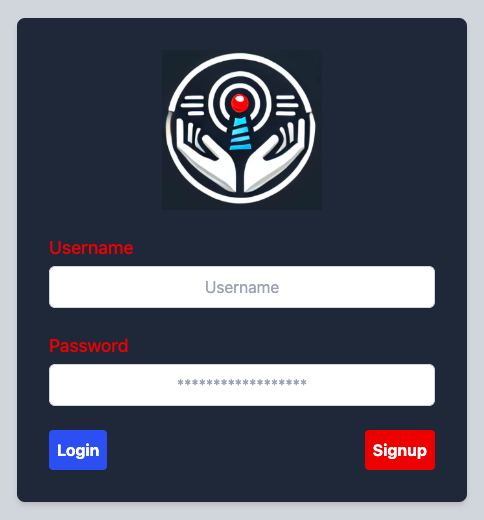
\includegraphics[width=0.3\textwidth]{img/login}
        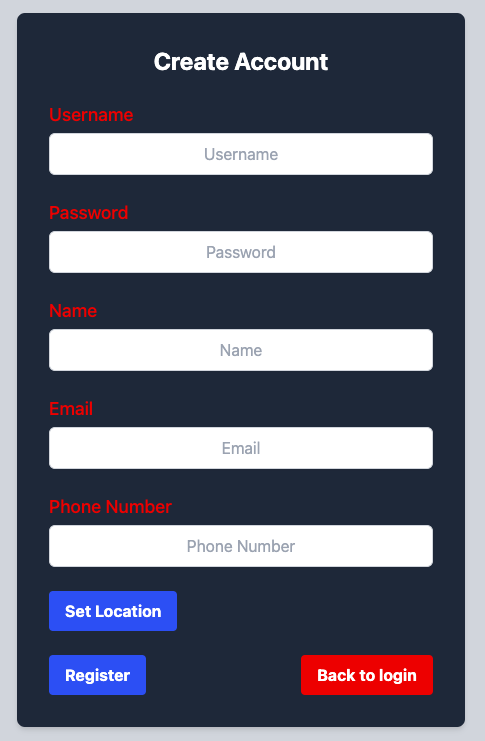
\includegraphics[width=0.3\textwidth]{img/register}
        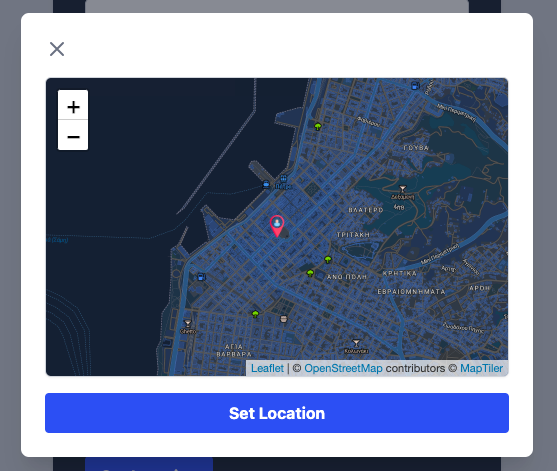
\includegraphics[width=0.3\textwidth]{img/register-location}
        \caption{Σελίδα Login - Register. \\Κατά την εγγραφή ορίζουμε την τοποθεσία του εκάστοτε χρήστη.}
    \end{figure}